\chapter{Dataset and Machine Learning}
The construction of the \emph{dataset} begins with the definition of the star cluster parameters, the galactic potential and the orbits, as well as the numerical integration conditions. The results are then analyzed through the distribution of the final quantities to study the relationship between the orbital parameters and the evolution of the clusters.
Based on this analysis, a binary classification problem is defined by establishing the criteria for distinguishing surviving clusters from dissolved ones, the input variables, and the division of the \emph{dataset} for training and evaluation. The \emph{F1-score}, used to measure classifier performance, is also introduced. Finally, the \emph{Support Vector Classifier} (SVC) and \emph{Multi-Layer Perceptron} (MLP) classifiers are presented, describing how they work and comparing their results.
\section{Dataset Generation}
\label{sec:costruzione-dataset}
The simulations are performed by varying the orbital parameters of the cluster, namely the semi-major axis and eccentricity. The results obtained constitute the \emph{dataset} used to study how different orbital conditions influence the evolution of star clusters.
\subsection{Star Cluster Parameters}
\label{subsec:condizioni-iniziali}
The star cluster is initialized according to the Plummer model, described in Section~\ref{subsec:plummer}. The number of stars, $\numberOfStars=200$, the scale parameter $\clusterRadius=1.0$, and the total mass $\totalMass=1.0$ are kept fixed in all simulations.
All stars have the same mass, calculated as:
\begin{equation}
	\starMass=\frac{\totalMass}{\numberOfStars}=0.005
	\label{eq:massa-singola-stella}
\end{equation}
To obtain different initial realizations of the cluster, 15 distinct random seeds are used, producing different initial distributions of stellar positions and velocities. This makes it possible to evaluate the influence of initial conditions on the results, avoiding basing the analysis on a single realization of the cluster.
\subsection{Galactic and Orbital Parameters}
\label{subsec:parametri-orbitali}
The external gravitational potential is described by the Plummer model, introduced in Section~\ref{subsec:plummer-galattico}, with a galactic mass of $\galaxyMass=3000.0$ and a scale parameter of $\galaxyRadius=20.0$, both kept constant across all simulations.
The orbits are defined by the semi-major axis $\semiMajorAxis$ and the eccentricity $\orbitEccentricity$. The former takes 30 values between $10.0$ and $300.0$, in increments of $10.0$:
\[
\semiMajorAxis \in \{10,20,30,\ldots,290,300\}
\]
The eccentricity takes 38 values between $0.0$ and $0.925$, in increments of $0.025$:
\[
\orbitEccentricity\in\{0,0.025,0.050,\ldots,0.900,0.925\}
\]
Considering all combinations of the two parameters yields $30\times38=1140$ orbital configurations. Each configuration is simulated using the 15 initial cluster realizations described in Section~\ref{subsec:condizioni-iniziali}. The \emph{dataset} therefore comprises a total of $15\times1140=17100$ simulations.
\subsection{Integration Parameters}
\label{subsec:parametri-integrazione}
The simulations use a gravitational constant of $\gravitationalConstant=1.0$, which allows all quantities to be expressed in a consistent system of units, avoiding conversions between different units of measurement. Numerical integration is performed using the \emph{leapfrog} method \cite{hairer2006geometric}, with a time step of $\deltat=0.005$. The softening parameter $\softeningLength$, introduced in Section~\ref{subsec:equazioni-moto}, is set to $0.01$.\\
The final simulation time is set to $\simulationEndTime=700.0$, in order to limit the influence of cluster dissolution caused by its internal dynamical evolution and focus on the effects of galactic tidal stripping \cite{cai2016evolution}.
\subsection{Summary of Parameters}
\label{subsec:riepilogo-parametri}
Table~\ref{tab:parametri-dataset} summarizes the parameters adopted for the simulations, distinguishing those kept constant from those varied to explore the different orbital configurations.
\begin{table}[H]
	\centering
	\caption{Parameters adopted for dataset generation.}
	\label{tab:parametri-dataset}
	\begin{tabular}{lll}
		\hline
		\textbf{Parameter} & \textbf{Symbol} & \textbf{Value} \\
		\hline
		\multicolumn{3}{l}{\textit{Star Cluster}} \\
		Number of stars & $\numberOfStars$ & $200$ \\
		Total mass & $\totalMass$ & $1.0$ \\
		Mass of a star & $\starMass$ & $0.005$ \\
		Plummer model scale parameter & $\clusterRadius$ & $1.0$ \\
		Number of random seeds used & --- & $15$ \\
		\hline
		\multicolumn{3}{l}{\textit{Galactic Potential}} \\
		Galactic mass & $\galaxyMass$ & $3000.0$ \\
		Galactic scale parameter & $\galaxyRadius$ & $20.0$ \\
		\hline
		\multicolumn{3}{l}{\textit{Orbital Parameters}} \\
		Semi-major axis & $\semiMajorAxis$ & $[10.0,\,300.0]$, step $10.0$ \\
		Eccentricity & $\orbitEccentricity$ & $[0.0,\,0.925]$, step $0.025$ \\
		\hline
		\multicolumn{3}{l}{\textit{Numerical Integration}} \\
		Gravitational constant & $\gravitationalConstant$ & $1.0$ \\
		Time step & $\deltat$ & $0.005$ \\
		Softening parameter & $\softeningLength$ & $0.01$ \\
		Final time & $\simulationEndTime$ & $700.0$ \\
		Integrator & --- & \emph{leapfrog} \\
		\hline
	\end{tabular}
\end{table}
\section{Dataset Analysis}
\label{sec:analisi-dataset}
\subsection{Distribution of Final Quantities}
\label{subsec:distribuzione-grandezze-finali}
To analyze the simulation results, we consider the histograms of the final bound mass fraction $\boundMassFraction$ and the ratio between the final half-mass radius $\halfMassRadius$ and its initial value $r_{1/2,0}$, defined as:
\begin{equation}
	\halfMassRadiusRatio = \frac{\halfMassRadius}{r_{1/2,0}}
	\label{eq:half-mass-radius-ratio}
\end{equation}
\begin{figure}[H]
	\centering
	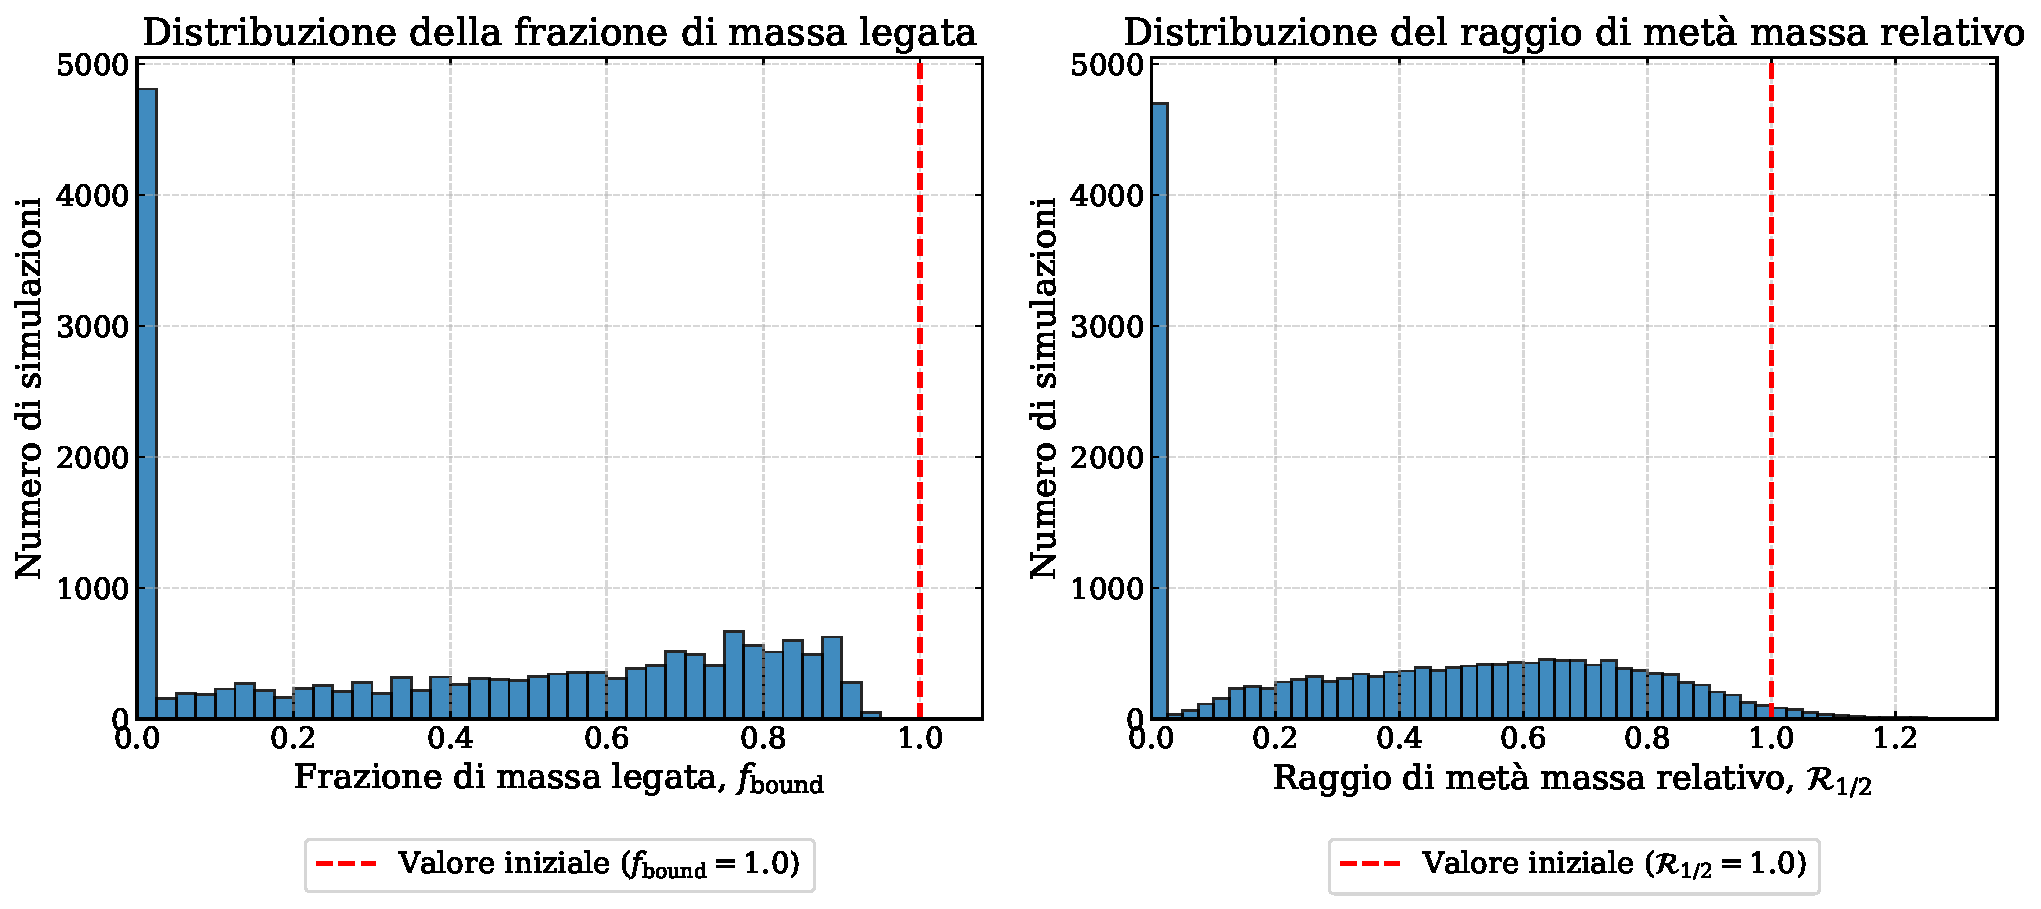
\includegraphics[width=\textwidth]{./plots/histogram_distribution_bmf_hmr.pdf}
	\caption{Distribution of the final bound mass fraction $\boundMassFraction$ (left) and the relative half-mass radius $\halfMassRadiusRatio$ (right).}
	\label{fig:distribuzione-grandezze-finali}
\end{figure}
\noindent Figure~\ref{fig:distribuzione-grandezze-finali} shows that both distributions exhibit a bimodal pattern, characterized by two distinct groups of values. In $4689$ simulations, corresponding to $27.42\%$ of the \emph{dataset}, both the bound mass fraction $\boundMassFraction$ and the relative half-mass radius $\halfMassRadiusRatio$ are zero. In these cases, no stars remain gravitationally bound to the cluster, and the stars have become completely dispersed under the effect of galactic tidal forces.\\ Outside the peak at zero, both distributions exhibit a flatter pattern, with values spread over a fairly wide range. However, most clusters have a bound mass fraction below $1.0$ and a relative half-mass radius also below $1.0$.\\ This indicates that, in most cases, the clusters have lost part of their mass and contracted relative to their initial configuration.\\ The two distributions are therefore consistent with each other, showing how mass loss is generally accompanied by a reduction in the cluster's spatial extent.
\subsection{Relationship Between Orbital Parameters and Simulation Outcomes}
\label{subsec:relazione-parametri-esiti}
Figure~\ref{fig:heatmap-bmf-hmr} shows the distributions of the final bound mass fraction $\boundMassFraction$ and the relative half-mass radius $\halfMassRadiusRatio$, as a function of the relative semi-major axis $\tilde{a}$ and the eccentricity $\orbitEccentricity$. The relative semi-major axis is defined as $\tilde{a}=\frac{\semiMajorAxis}{\galaxyRadius}$ and is a dimensionless quantity expressing the orbital extent in units of the galactic scale parameter $\galaxyRadius$. Each cell represents the mean of the results from the $15$ initial realizations for a given orbital configuration.
\begin{figure}[H]
	\centering
	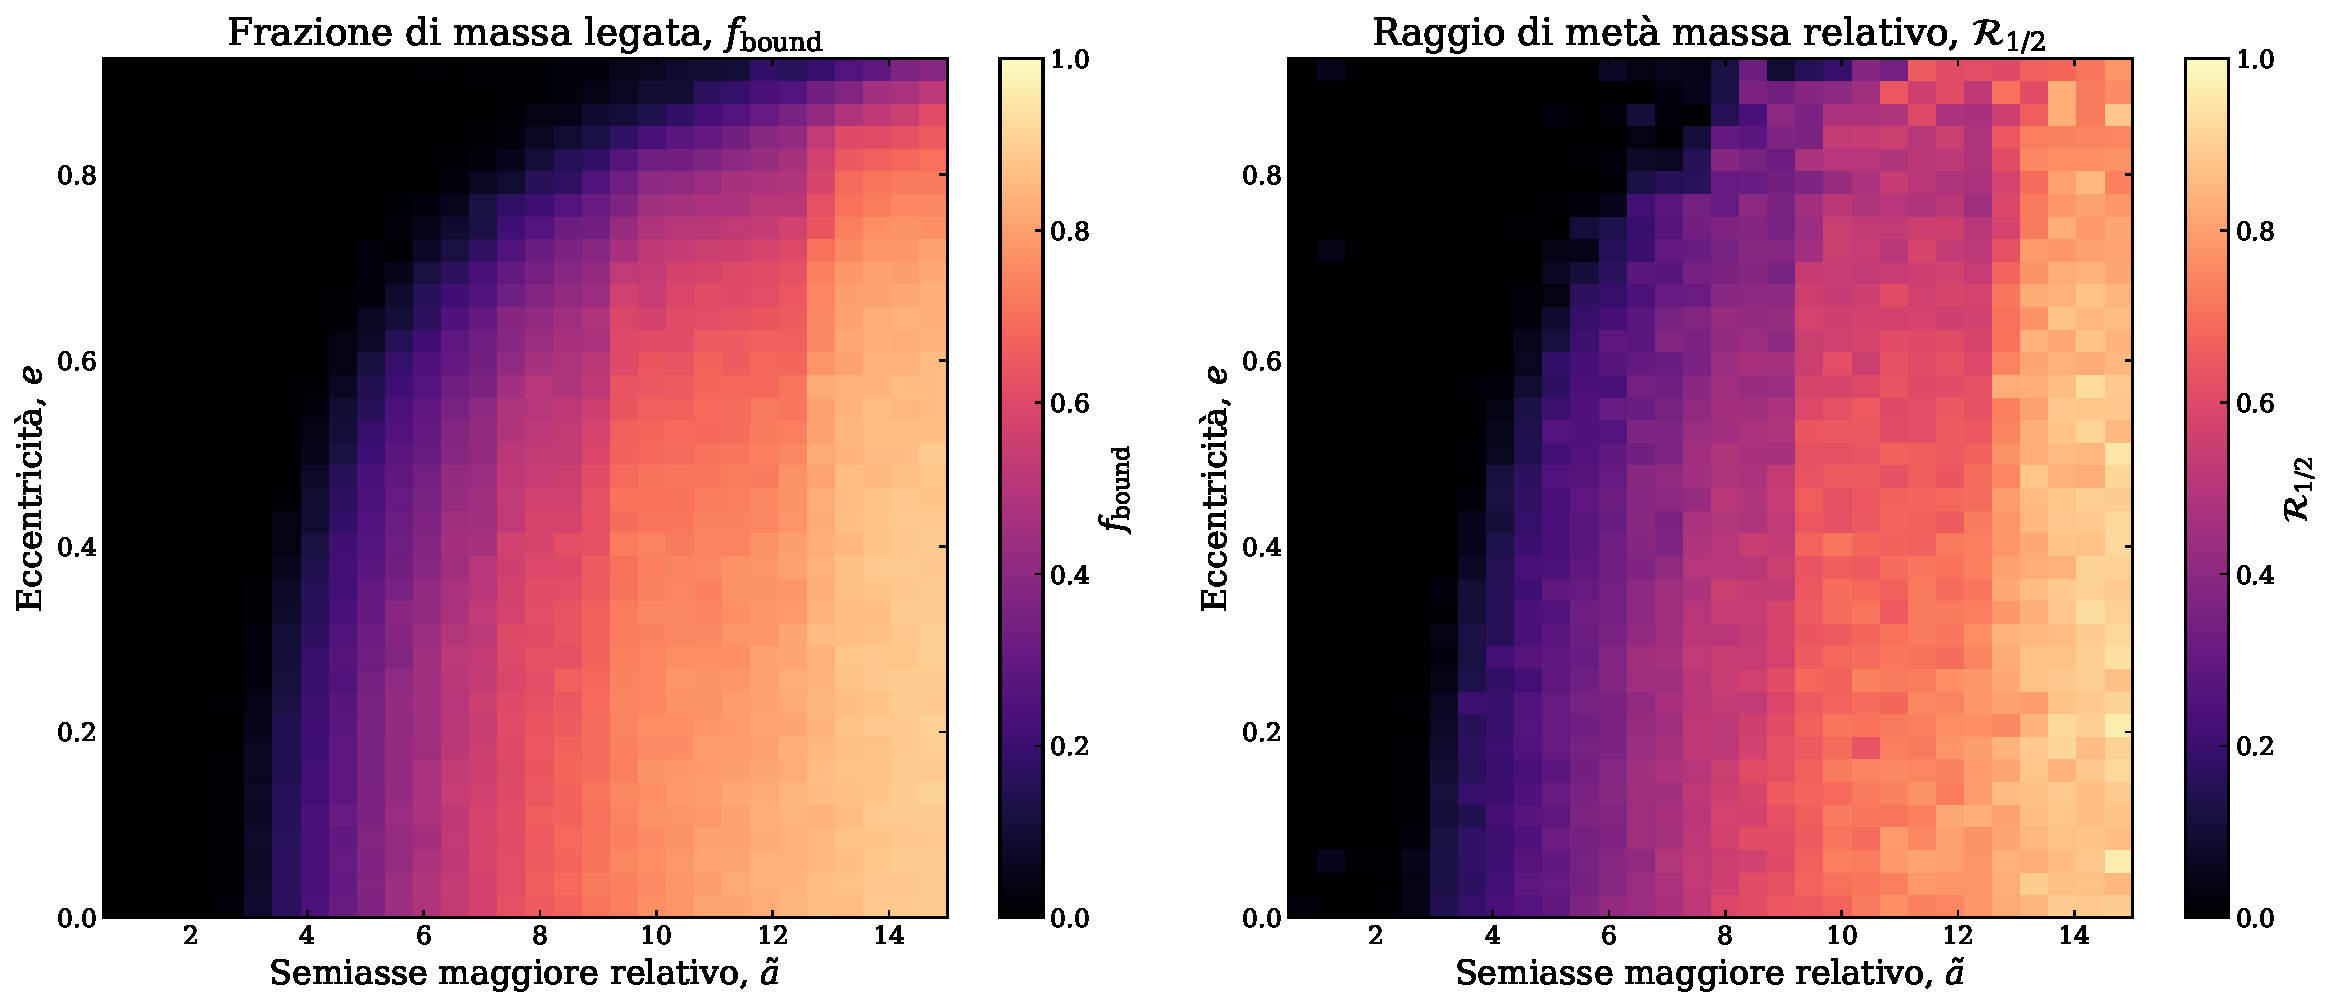
\includegraphics[width=\textwidth]{./plots/heat_distribution_bmf_hmr.pdf}
	\caption{Distribution of the mean values of the final bound mass fraction $\boundMassFraction$ (left) and the relative half-mass radius $\halfMassRadiusRatio$ (right), as a function of the relative semi-major axis $\tilde{a}$ and the eccentricity $\orbitEccentricity$.}
	\label{fig:heatmap-bmf-hmr}
\end{figure}
\noindent The distributions reveal a clearly identifiable transition line between orbital configurations for which the bound mass fraction and the relative half-mass radius are zero or close to zero, and those in which both quantities remain positive. This separation provides further evidence of the relationship between the values of the quantities describing the cluster's state and its evolution.\\ In particular, for relative semi-major axis values below approximately $3.0$, both quantities tend to approach zero, indicating the complete dissolution of the cluster due to the greater intensity of tidal effects at smaller distances from the galactic center.\\ Eccentricity also affects the evolution of the cluster: for the same semi-major axis, higher values result in a smaller distance from the galactic center at pericenter, exposing the cluster to stronger tidal effects and promoting its dissolution.
\section{Definition of the Classification Problem}
\label{sec:definizione-problema-di-classificazione}
To apply machine learning methods, the \emph{dataset} is organized into a set of input variables and a set of labels, defining the criteria for assigning classes and the subsequent division of the data for model training and evaluation.
\subsection{Classification of Star Clusters}
\label{subsec:classificazione-ammassi}
As shown in Section~\ref{subsec:distribuzione-grandezze-finali}, at the end of the simulation star clusters can exhibit different evolutionary outcomes: some retain a compact, gravitationally bound structure, while others undergo mass loss and changes in spatial extent that significantly alter their initial structure. These differences make it possible to distinguish two classes of evolutionary outcome: surviving clusters and dissolved clusters. In this work, this distinction is used to formulate a binary classification problem, in which each cluster is assigned a label corresponding to its class.
\begin{figure}[H]
	\centering
	\begin{minipage}[t]{0.48\textwidth}
		\centering
		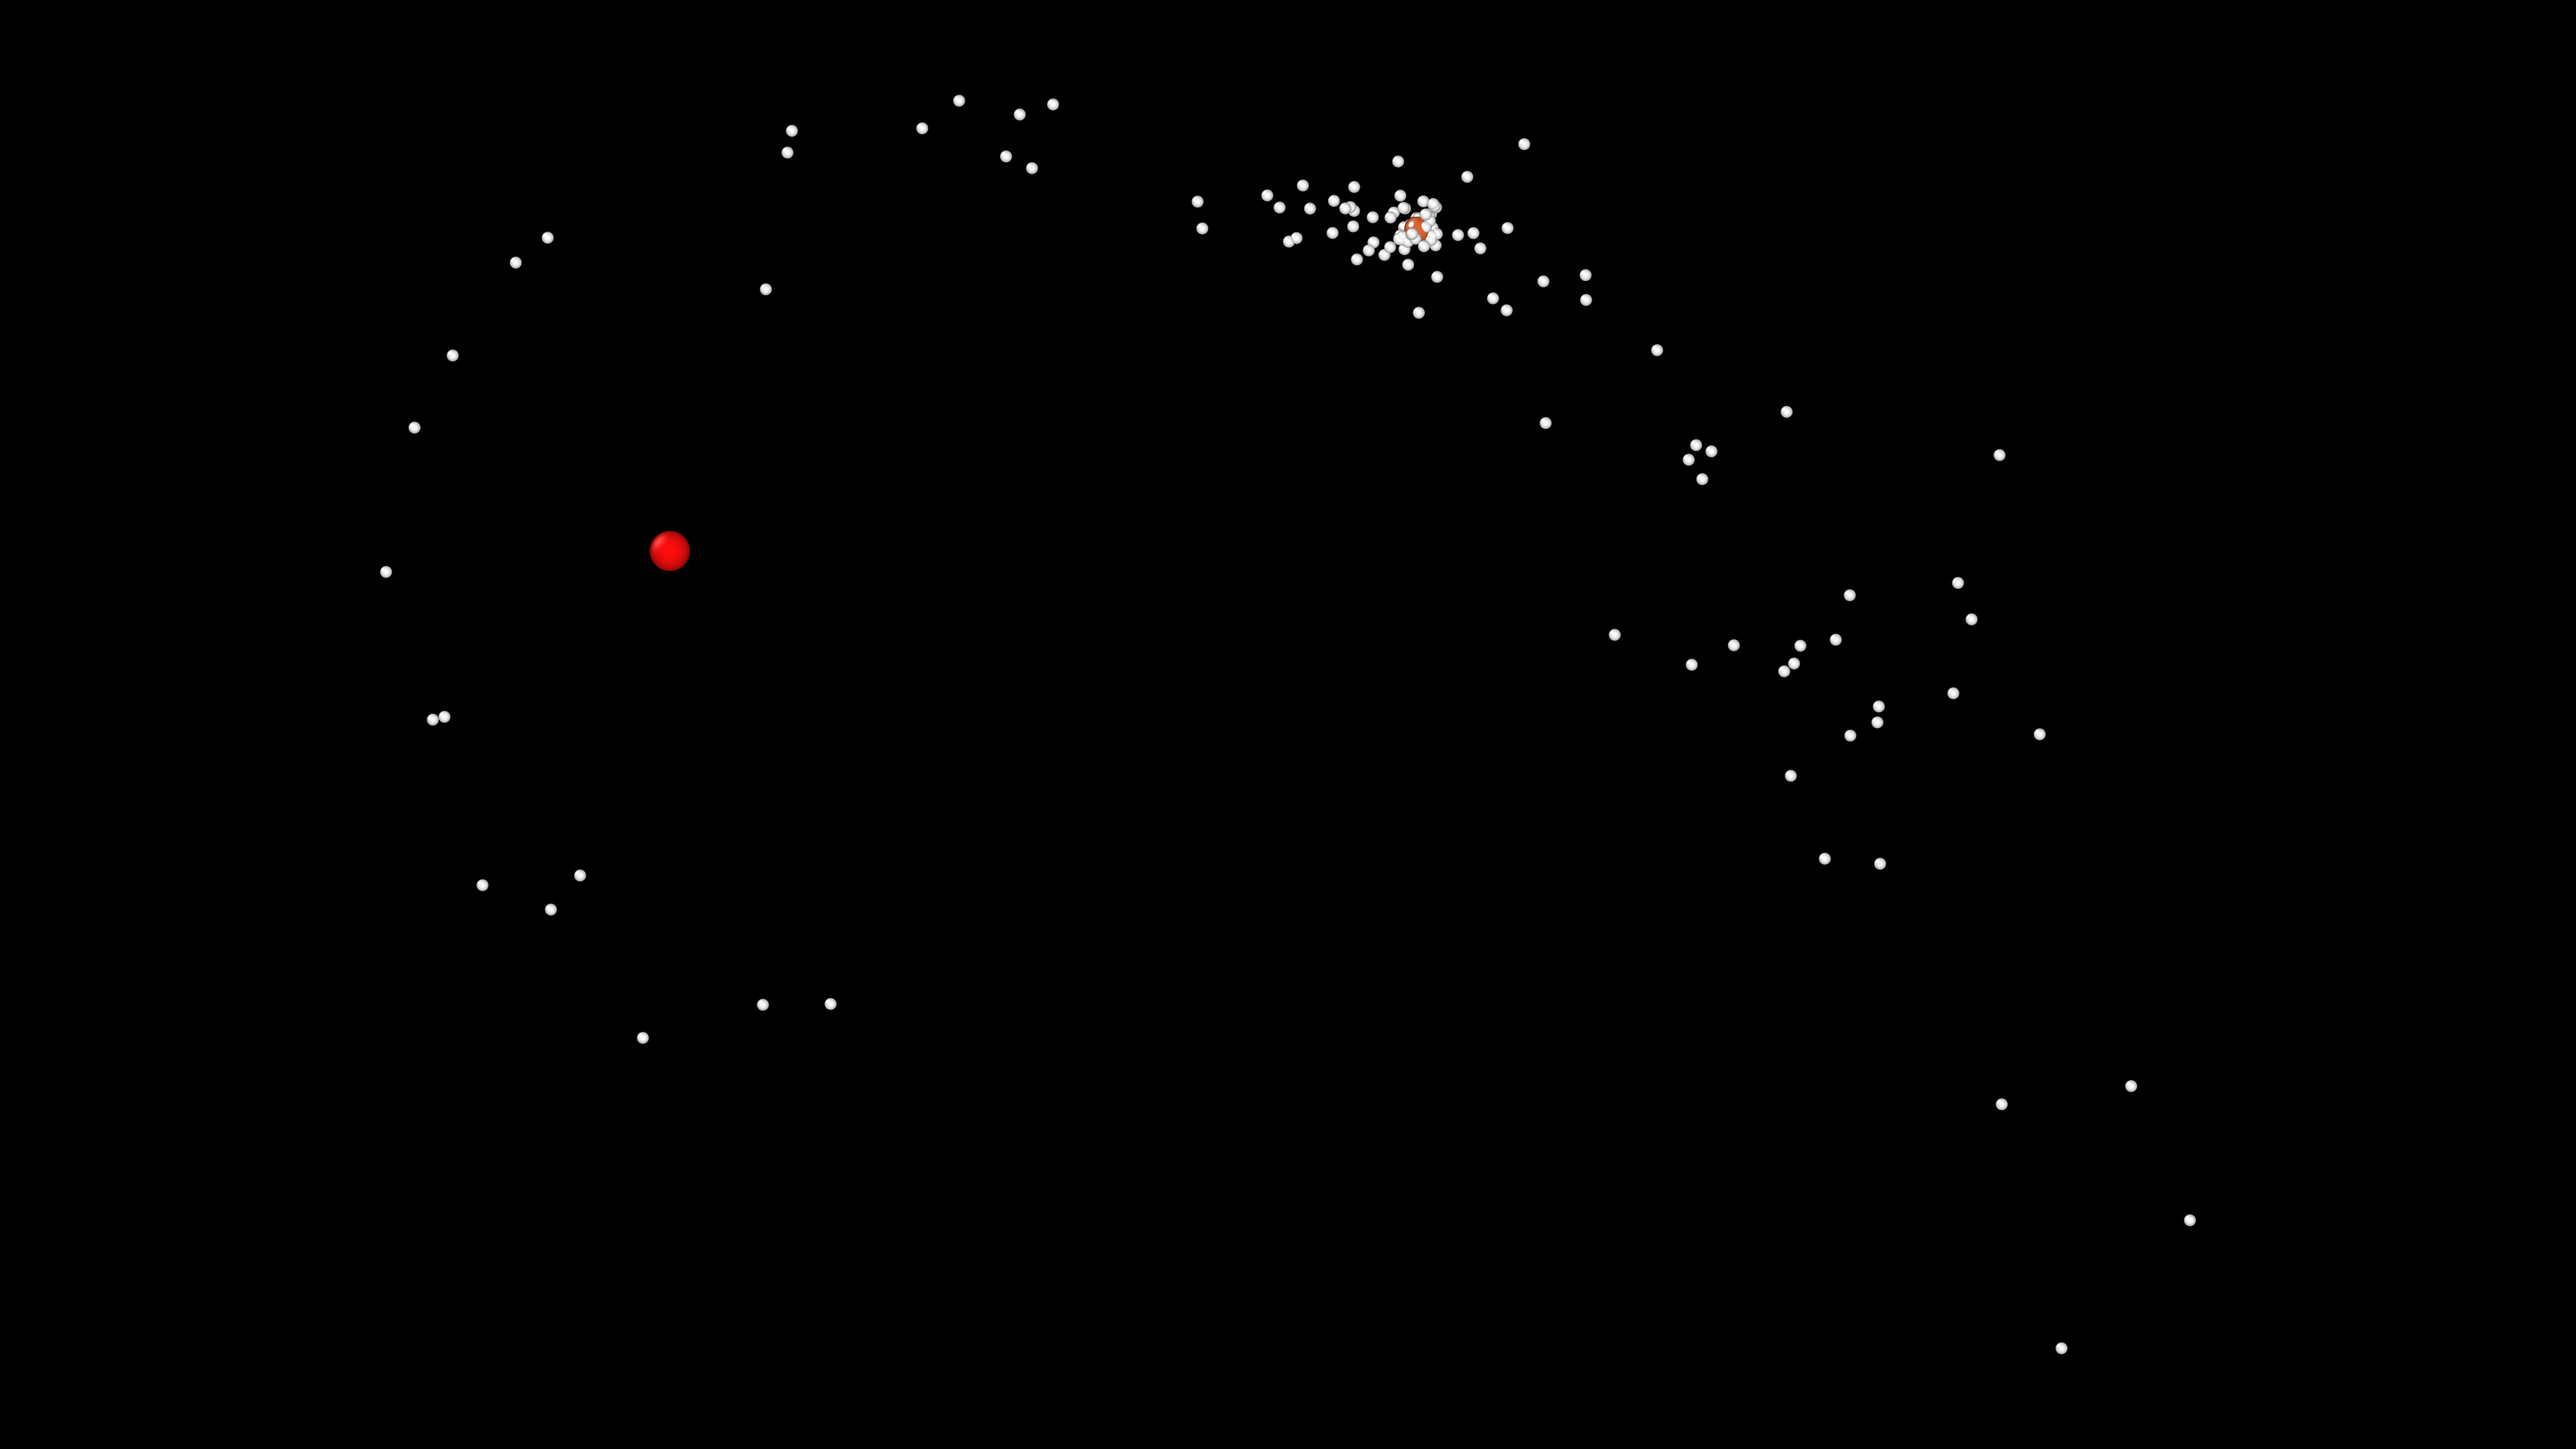
\includegraphics[width=\textwidth]{./images/cluster_alive.png}
		\vspace{0.3em}
		\small Surviving star cluster \\ ($\semiMajorAxis = 300.0$, $\orbitEccentricity = 0.5$) \\ ($\boundMassFraction = 0.93$, $\halfMassRadiusRatio = 1.002$)
	\end{minipage}
	\hfill
	\begin{minipage}[t]{0.48\textwidth}
		\centering
		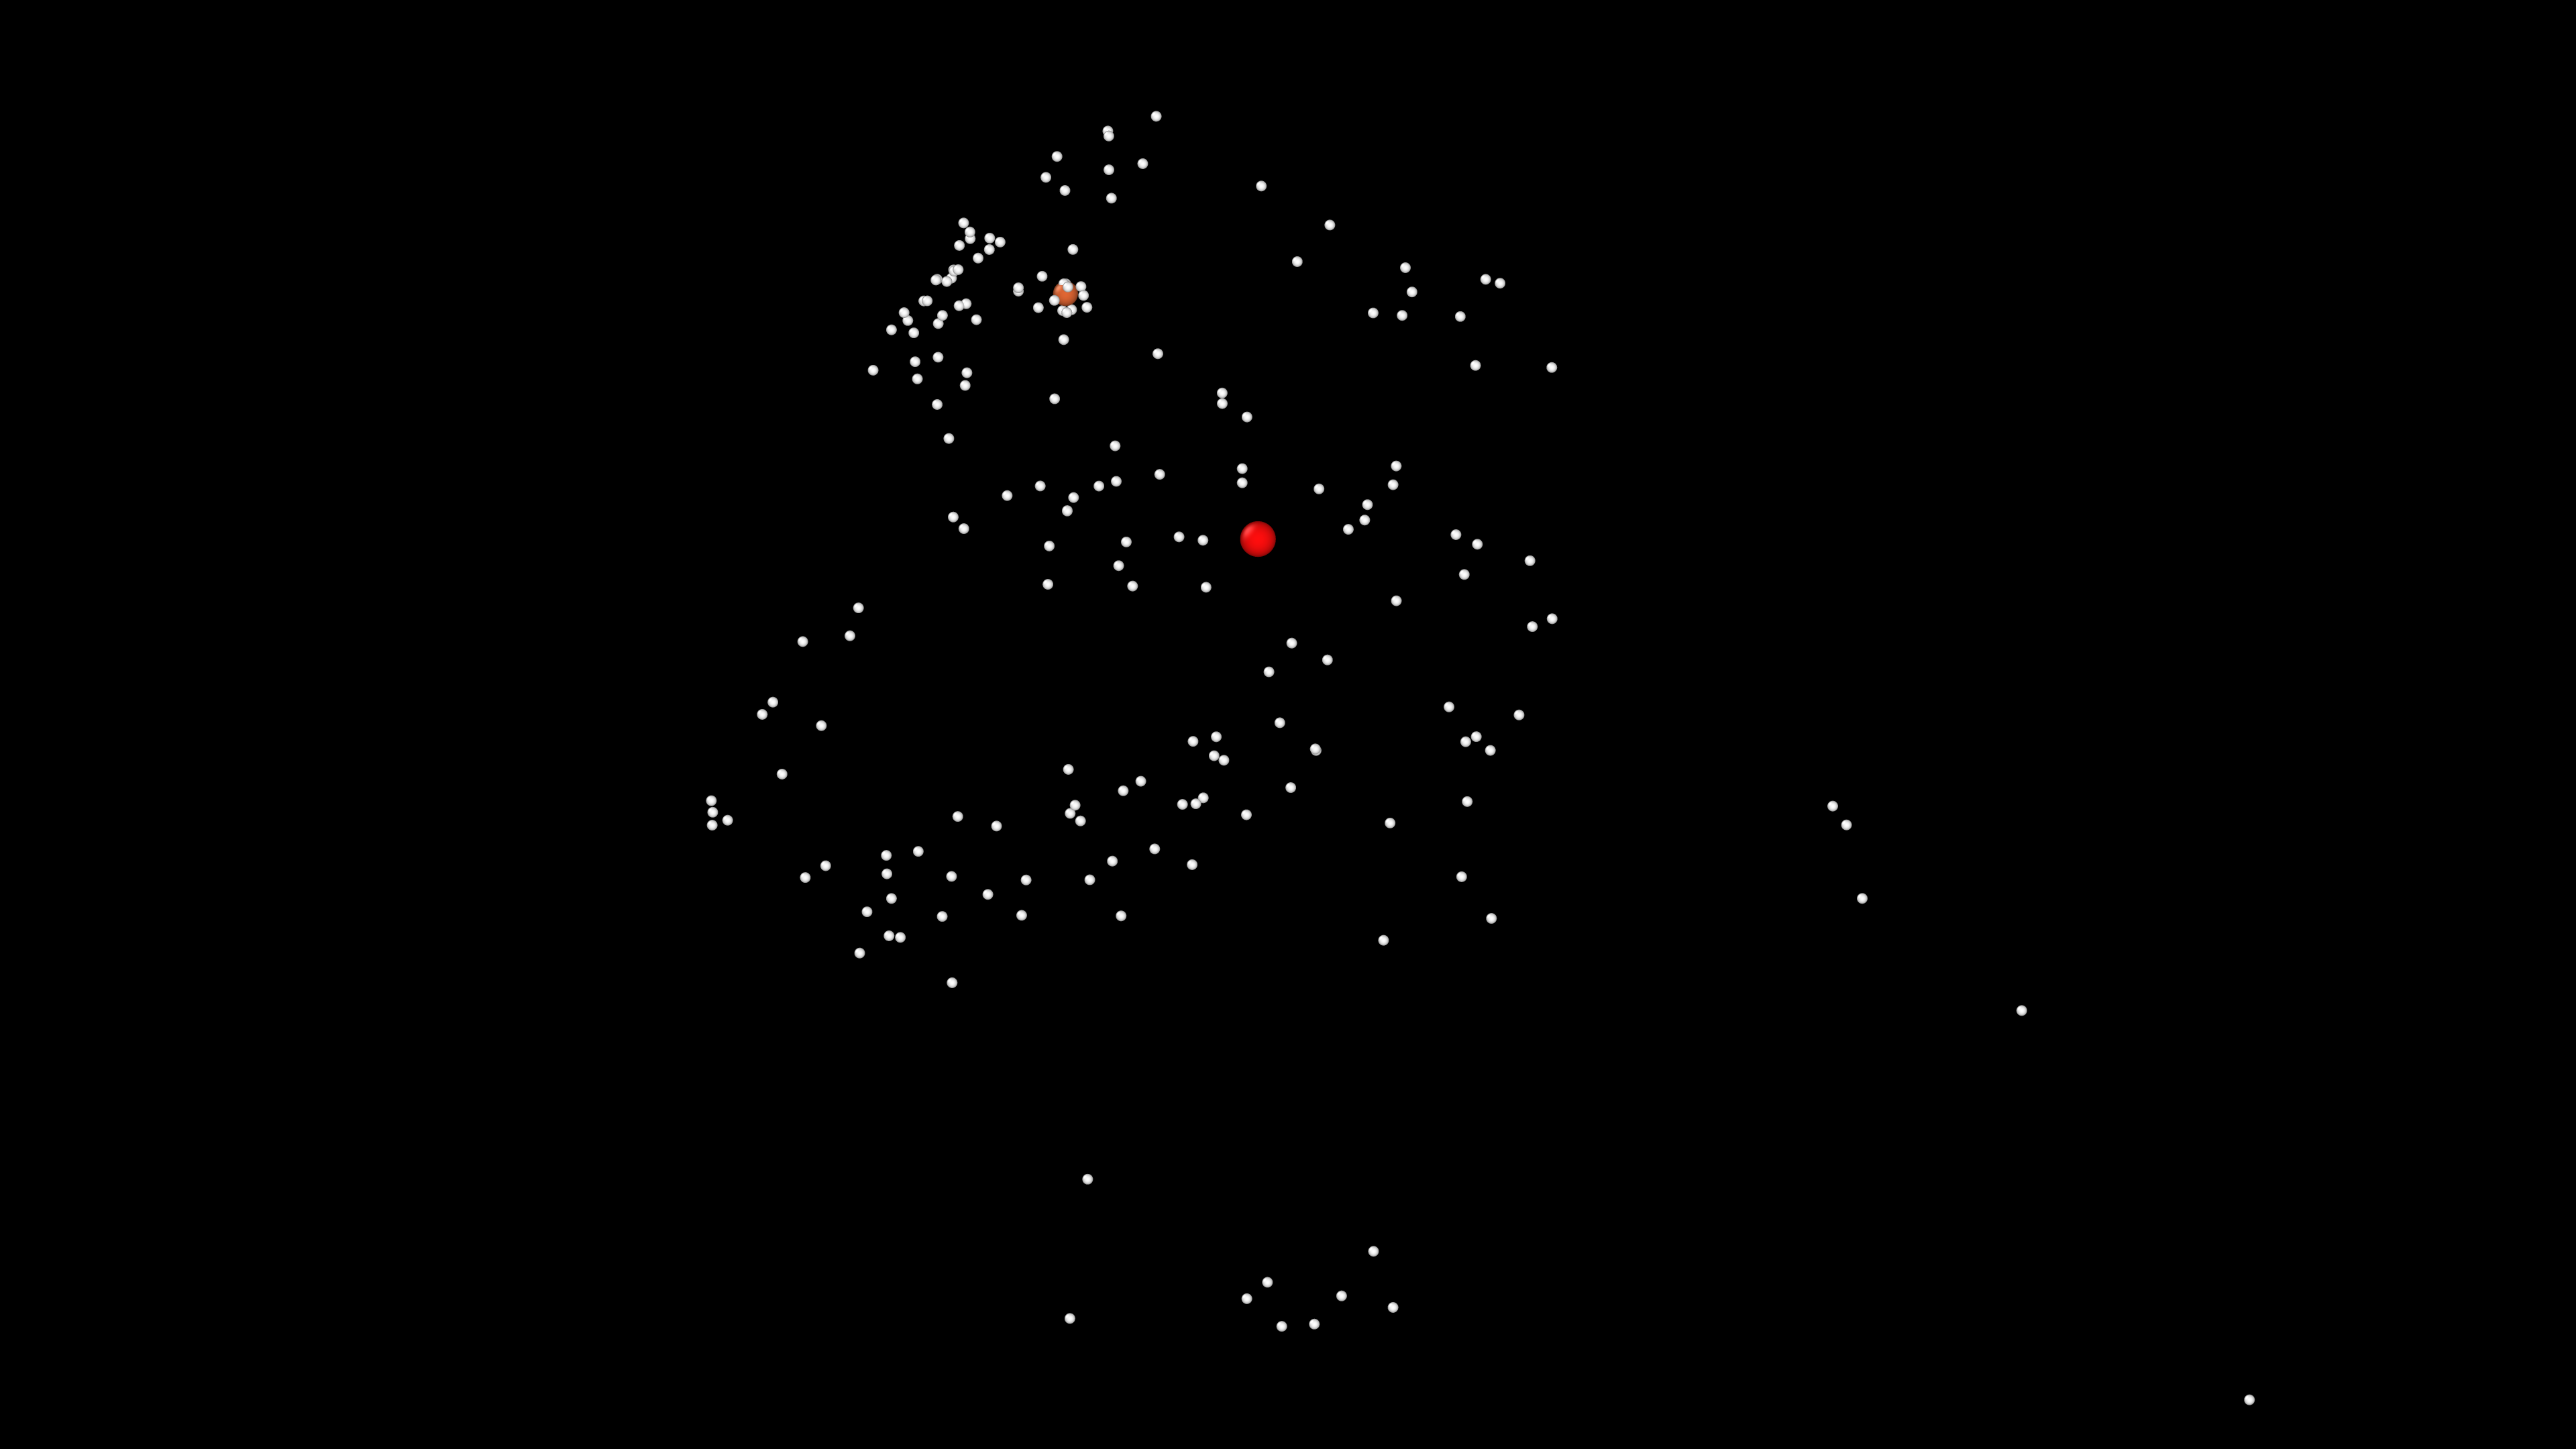
\includegraphics[width=\textwidth]{./images/cluster_dead.png}
		\vspace{0.3em}
		\small Dissolved star cluster \\ ($\semiMajorAxis = 140.0$, $\orbitEccentricity = 0.8$) \\ ($\boundMassFraction = 0.065$, $\halfMassRadiusRatio = 0.246$)
	\end{minipage}
	\caption{Evolution of the same star cluster, generated from the same initial configuration and subjected to different orbital conditions. The images show the configurations reached at time $\simulationEndTime$: in one case the cluster survives, while in the other it dissolves. The configurations are visualized using OVITO \cite{stukowski2010}: stars are shown in white, the galactic center in red, and the center of mass of the bound stars in orange.\\ ($\numberOfStars = 200$, $\clusterRadius = 1.0$, $\galaxyMass = 3000.0$, $\galaxyRadius = 20.0$, $\gravitationalConstant = 1.0$, $\softeningLength = 0.01$, $\deltat = 0.005$, $\simulationEndTime = 700.0$, \emph{leapfrog})}
	\label{fig:esempi-ammassi}
\end{figure}
\subsection{Formal Definition of the Sets}
\label{subsec:criterio-vivi-morti}
Let $\allClusters$ be the set of all star clusters $i$. As described in Section~\ref{subsec:classificazione-ammassi}, the clusters are divided into two subsets, $\aliveCluster$ and $\deadCluster$, containing the surviving and dissolved clusters, respectively. This division is based on two quantities associated with each cluster $i$: the bound mass fraction $f_{\mathrm{bound}, i}$ and the ratio between the final and initial half-mass radii $\mathcal{R}_{1/2, i}$. The adopted threshold values are $0.1$ for the bound mass fraction and $0.2$ for the relative half-mass radius. These thresholds were identified through an analysis of the cluster configurations in the initial and final stages of the simulations, as well as of the distributions of the final quantities presented in Sections~\ref{subsec:distribuzione-grandezze-finali} and~\ref{subsec:relazione-parametri-esiti}.
The sets $\aliveCluster$ and $\deadCluster$ are defined as follows:
\[
\aliveCluster = \left\{ i \in \allClusters \,\middle|\, f_{\mathrm{bound}, i} > 0.1 \;\land\; \mathcal{R}_{1/2, i} > 0.2 \right\}
\]
\[
\deadCluster = \left\{ i \in \allClusters \,\middle|\, f_{\mathrm{bound}, i} \leq 0.1 \;\lor\; \mathcal{R}_{1/2, i} \leq 0.2 \right\}
\]
The two sets are disjoint and exhaustive with respect to $\allClusters$, since they satisfy the following properties:
\[
\aliveCluster \cap \deadCluster = \emptyset
\qquad
\aliveCluster \cup \deadCluster = \allClusters.
\]
Out of a total of $|\allClusters|=17\,100$ analyzed simulations, the set $\aliveCluster$ contains 11\,695 clusters, corresponding to $68.39\%$ of the total, while $\deadCluster$ contains 5\,405 clusters, corresponding to $31.61\%$.
\subsection{Input and Output Variables}
\label{subsec:variabili-ingresso-uscita}
For each simulation, the input variable vector is defined as
\begin{equation}
	\mathbf{x} =
	\begin{bmatrix}
		\semiMajorAxis \\
		\orbitEccentricity
	\end{bmatrix}
\end{equation}
These parameters describe the initial orbital conditions and constitute the information available to the model for predicting the simulation outcome.
Considering all simulations, the input matrix is represented by
\begin{equation}
	X \in \mathbb{R}^{|\allClusters|\times 2}
\end{equation}
while the labels associated with the simulations form the vector
\begin{equation}
	Y \in \{0,1\}^{|\allClusters|}
\end{equation}
Using the sets $\aliveCluster$ and $\deadCluster$, defined in Section~\ref{subsec:criterio-vivi-morti}, each simulation $i$ is assigned a label according to the following definition:
\begin{equation}
	Y_i =
	\begin{cases}
		1 & \text{if } i \in \aliveCluster\\
		0 & \text{if } i \in \deadCluster
	\end{cases}
\end{equation}
\begin{figure}[H]
	\centering
	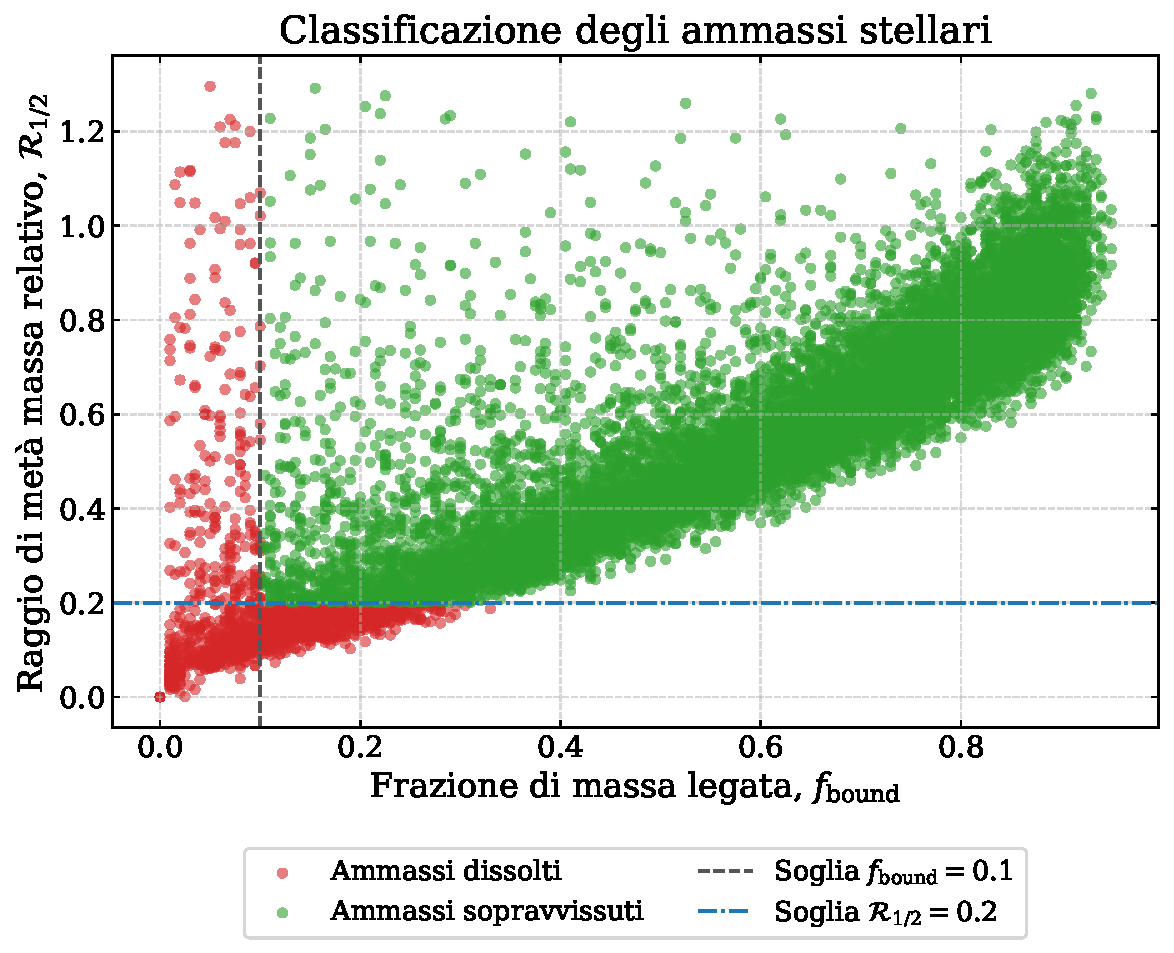
\includegraphics[width=0.75\textwidth]{plots/cluster_classification.pdf}
	\caption{Outcome of the binary classification of star clusters.}
	\label{fig:distribuzione-ammassi}
\end{figure}
\subsection{Training and Test Set Split}
\label{subsec:suddivisione-dataset}
To evaluate the models' ability to generalize, the \emph{dataset} is randomly divided into a training set containing 80\% of the simulations and a test set containing the remaining 20\%. Thus, out of a total of $17100$ simulations, there are $13680$ training samples and $3420$ evaluation samples. The split is stratified by labels, so as to maintain comparable proportions of surviving and dissolved clusters in the two sets. Sample selection is performed using a pseudo-random procedure controlled by a predefined seed, kept identical for both models. This ensures that the two splits are the same and that the results are comparable and reproducible.
The \emph{training set} is used to learn the relationship between the orbital parameters and the labels, while the \emph{test set} is used exclusively to evaluate model performance on simulations not used during training.
\subsection{Comparison Using the F1-score}
\label{subsec:confronto-f1-score}
To evaluate model performance, precision and recall are considered. These are two complementary measures that describe, respectively, the reliability of predictions and the ability to correctly identify elements belonging to a given class. Both are calculated separately for surviving and dissolved clusters.\\ Let $TP$ denote the number of elements belonging to the considered class that are correctly classified, $FP$ the number of elements belonging to the other class but incorrectly assigned to the considered class, and $FN$ the number of elements belonging to the considered class but incorrectly assigned to the other class. The resulting measures are:
\begin{equation}
	\mathrm{Precision} = \frac{TP}{TP+FP}
	\label{eq:precisione}
\end{equation}
\begin{equation}
	\mathrm{Recall} = \frac{TP}{TP+FN}
	\label{eq:richiamo}
\end{equation}
To summarize both measures in a single value, the \emph{F1-score} is used, defined as their harmonic mean \cite{sokolova2009systematic}:
\begin{equation}
	\mathrm{F1\text{-}score} = 2 \cdot \frac{\mathrm{Precision}\cdot\mathrm{Recall}}{\mathrm{Precision}+\mathrm{Recall}}
	\label{eq:f1-score}
\end{equation}
The \emph{F1-score} is therefore calculated separately for each class and takes values between $0$ and $1$: values closer to $1$ indicate a more accurate classification. Finally, to obtain an overall measure of performance, the weighted average of the \emph{F1-scores} of the two classes is used, with each contribution proportional to the number of simulations belonging to the respective class.
\section{Application of the Models}
\label{sec:applicazione-modelli}
In this section, two machine learning models are applied to classify star clusters based on their initial orbital parameters. The models considered are a \emph{Support Vector Classifier} and a \emph{Multi-Layer Perceptron} neural network, whose main characteristics are described. Both are trained using the \emph{training set} data and subsequently evaluated on the \emph{test set}, comparing their performance.
\subsection{Feature Standardization}
\label{subsec:standardizzazione-variabili}
Before training, the input variables are standardized to make them comparable, preventing differences in their numerical ranges from influencing the learning process.\\ The transformation applied to each variable is:
\begin{equation}
	x' = \frac{x-\mu}{\sigma}
	\label{eq:standardizzazione}
\end{equation}
where $x$ is the original value, while $\mu$ and $\sigma$ denote the mean and standard deviation, respectively. These parameters are calculated exclusively on the \emph{training set} and subsequently used to transform the \emph{test set} as well. This prevents information contained in the test data from indirectly influencing model training \cite{kaufman2012leakage}.
\subsection{Support Vector Classifier}
\label{subsec:svc}
\subsubsection{Model}
The first classifier used is the \emph{Support Vector Classifier} (SVC), based on \emph{Support Vector Machines} (SVM) \cite{cortes1995support}. Its objective is to identify a decision boundary that separates surviving clusters from dissolved ones in the space defined by the orbital parameters. The position of this boundary depends primarily on the samples closest to it, called support vectors, which determine its shape.
To allow for non-linear separation, a second-degree polynomial kernel is adopted, defined as:
\begin{equation}
	K(\mathbf{x},\mathbf{z})=(\gamma\,\mathbf{x}\cdot\mathbf{z}+r)^2
	\label{eq:svc-polynomial-kernel}
\end{equation}
A kernel makes it possible to evaluate the relationship between two samples through a mathematical function, allowing decision boundaries to be identified even when the classes cannot be separated by a simple straight line \cite{scholkopf2002learning}. In this expression, $\mathbf{x}$ and $\mathbf{z}$ represent two vectors containing the standardized orbital parameters, while $\mathbf{x}\cdot\mathbf{z}$ denotes their dot product.\\
The parameter $\gamma$ determines the scale of the dot product and is calculated according to the following relation \cite{scikitlearnsvmdoc}:
\begin{equation}
	\gamma = \frac{1}{n_{\mathrm{feature}}\cdot\operatorname{Var}(X)}
	\label{eq:svc-gamma}
\end{equation}
where $n_{\mathrm{feature}}$ denotes the number of input variables and $\operatorname{Var}(X)$ their average variance. Since the two variables have been standardized (Section~\ref{subsec:standardizzazione-variabili}), their variance is equal to one. Therefore:
\[
\gamma = \frac{1}{2\cdot 1}=0.5
\]
The parameter $r$, corresponding to the constant term of the kernel, is set to $1.0$. This choice makes it possible to include, in addition to quadratic terms and interactions between the variables, linear terms and a constant term. Substituting this value into Equation~\ref{eq:svc-polynomial-kernel} gives:
\begin{equation}
	K(\mathbf{x},\mathbf{z}) =
	\gamma^2(\mathbf{x}\cdot\mathbf{z})^2
	+2\gamma(\mathbf{x}\cdot\mathbf{z})+1
	\label{eq:svc-polynomial-kernel-expanded}
\end{equation}
\subsubsection{Results}
\begin{figure}[H]
	\centering
	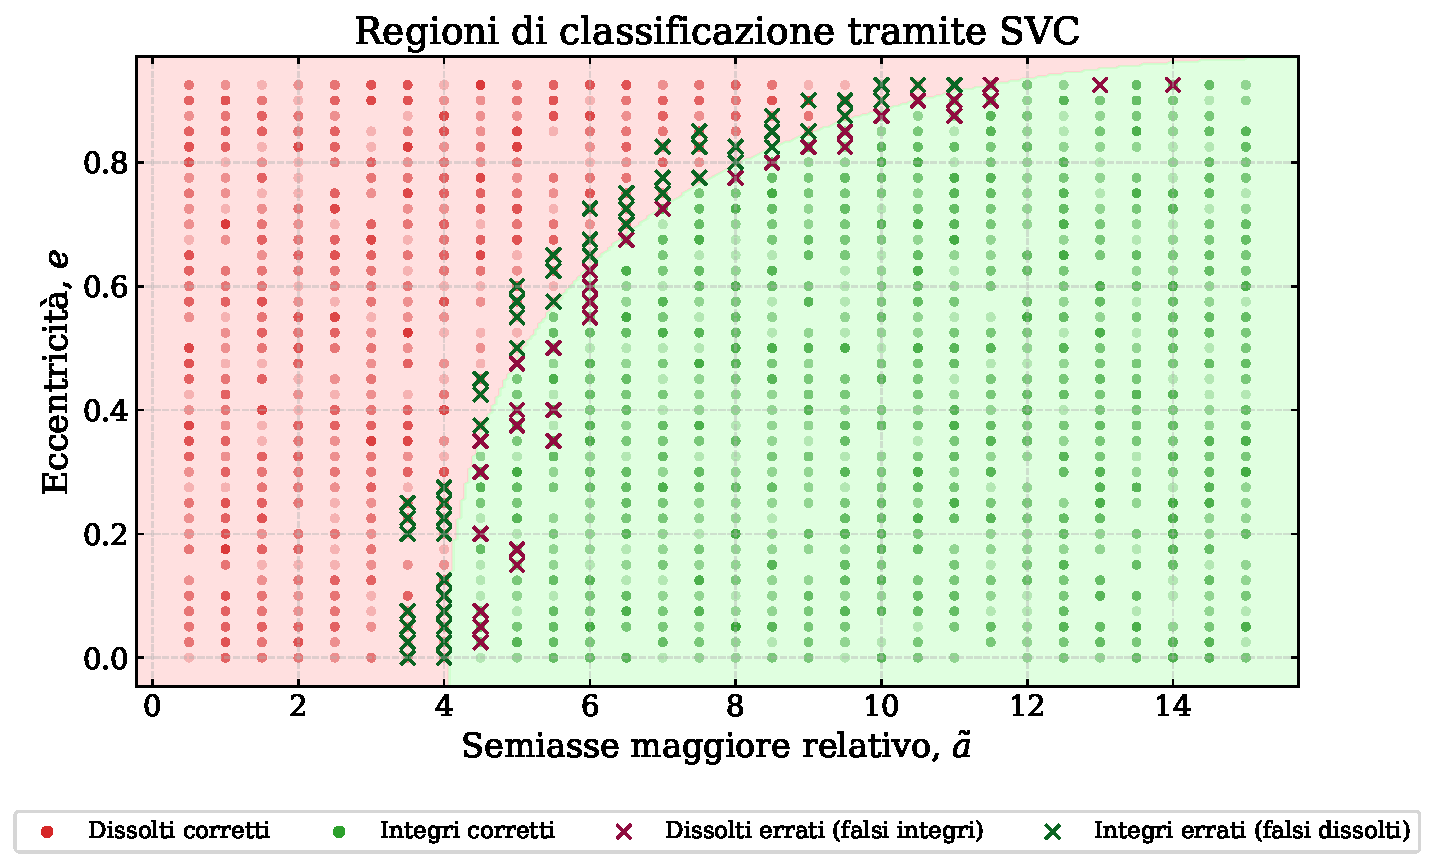
\includegraphics[width=0.8\textwidth]{plots/svc_decision_boundaries.pdf}
	\caption{Decision regions of the SVC classifier as a function of the relative semi-major axis $\tilde{a}$ and eccentricity $\orbitEccentricity$. The background represents the model predictions, while the points show the \emph{test set} simulations; crosses indicate misclassifications. (\emph{F1-score} = 0.9644)}
	\label{fig:svc-decision-boundaries}
\end{figure}
On the \emph{test set}, the classifier achieves a weighted \emph{F1-score} of $0.9644$. Performance is high for both classes, with a value of $0.95$ for dissolved clusters and $0.97$ for surviving clusters.
Thanks to the expanded form of the kernel, described in Equation~\ref{eq:svc-polynomial-kernel-expanded}, the decision boundary can be expressed through an explicit quadratic equation.\\
Expressing the coefficients in the original orbital parameter space gives:
\begin{equation}
	\begin{aligned}
		f(a, e) = \, & -0.0001\,a^2
		- 9.1336\,e^2
		- 0.0747\,ae
		+ 0.1614\,a
		+ 6.4634\,e
		- 12.1809
	\end{aligned}
	\label{eq:svc-decision-boundary}
\end{equation}
Considering the coefficients alone, they might appear to indicate a greater influence of eccentricity on the classification, since the terms containing it have larger absolute values. However, it must be taken into account that the semi-major axis assumes numerically much larger values than eccentricity. The different numerical scales of the two parameters are therefore reflected in the coefficients learned by the model, which has identified a relationship involving both parameters and their combination in determining the classification outcome.
\begin{figure}[H]
	\centering
	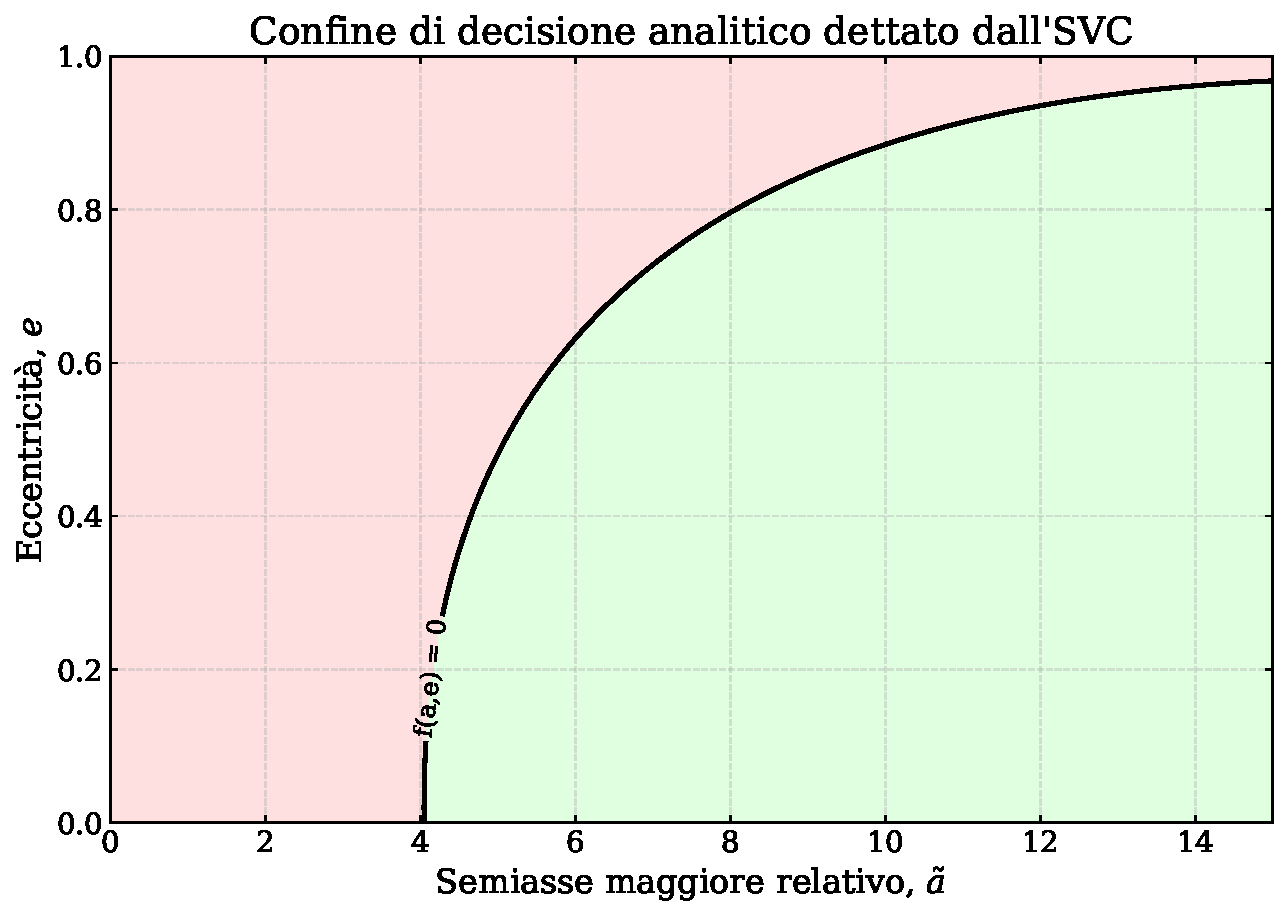
\includegraphics[width=0.7\textwidth]{plots/svc_analytical_boundary.pdf}
	\caption{Graphical representation of the decision boundary defined by Equation~\ref{eq:svc-decision-boundary}.\\ The green region represents the cluster survival zone ($f(a,e)>0$), while the red region represents the dissolution zone ($f(a,e)<0$).}
	\label{fig:svc-analytical-boundary}
\end{figure}
\subsection{Multi-Layer Perceptron}
\label{subsec:mlp}
\subsubsection{Model}
The second classifier used is a \emph{Multi-Layer Perceptron} (MLP), an artificial neural network composed of neurons arranged in different layers \cite{goodfellow2016deeplearning}. Each neuron receives the values produced by the previous layer, combines them using numerical weights, and returns an output that is passed to the subsequent neurons. During training, these weights are adjusted to improve the model's ability to correctly classify the clusters \cite{rumelhart1986learning}.
The adopted architecture comprises two hidden layers, containing 16 and 8 neurons, respectively, and an output layer for binary classification. The hidden layers use the ReLU (\emph{Rectified Linear Unit}) activation function, defined as:
\[
\operatorname{ReLU}(x)=\max(0,x)
\]
This function returns zero for negative values and leaves positive values unchanged. Its introduction allows the network to learn non-linear relationships between the input variables \cite{glorot2011rectifier}.\\
Weight updates during training are performed by the Adam algorithm, an optimization method that automatically adjusts the magnitude of the updates based on the errors made by the network and the behavior of the gradients across iterations \cite{kingma2015adam}.\\ Training consists of a maximum of 500 iterations.
\subsubsection{Results}
\begin{figure}[H]
	\centering
	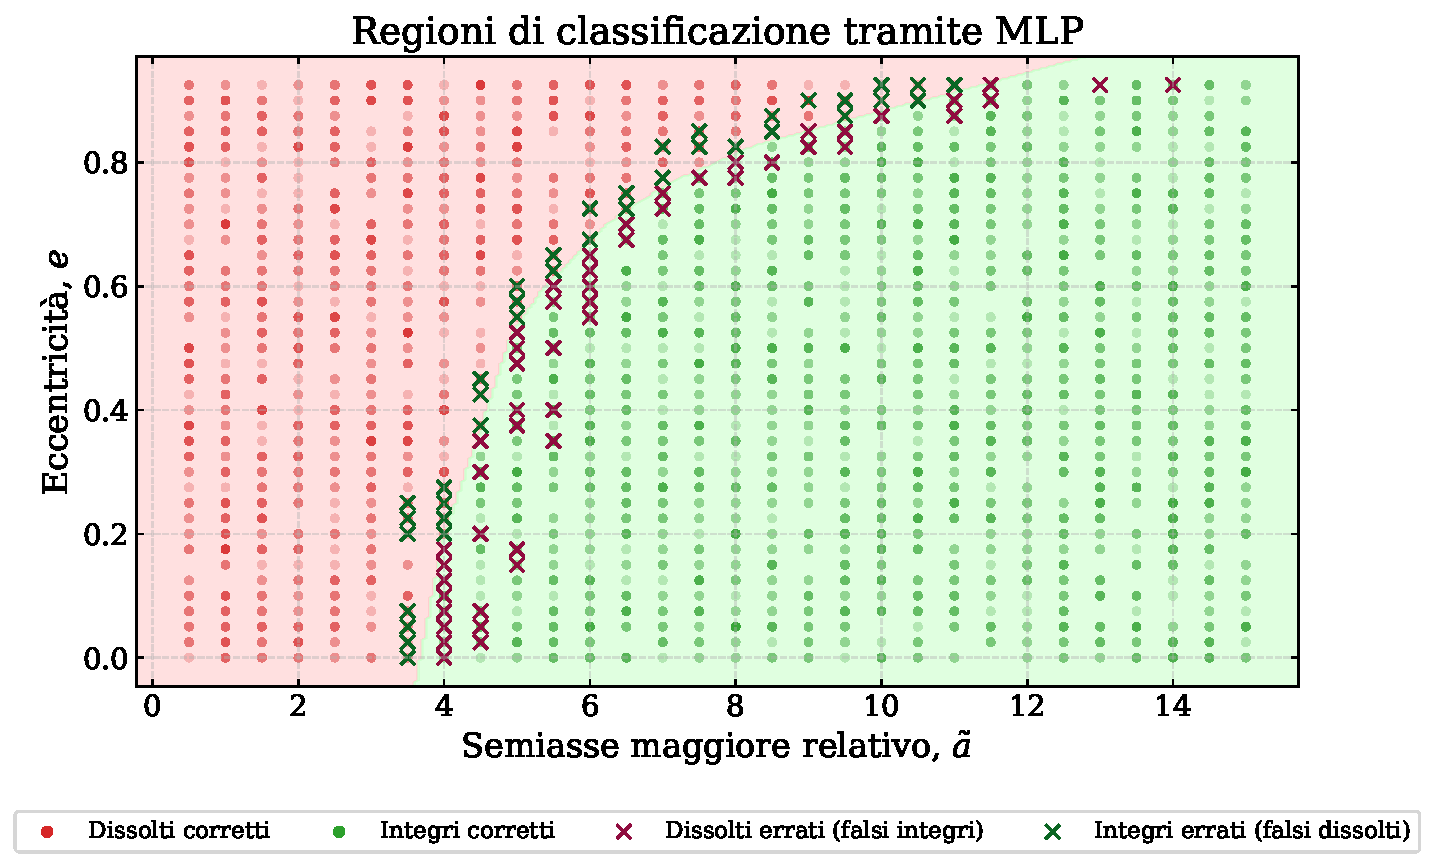
\includegraphics[width=0.8\textwidth]{plots/mlp_decision_boundaries.pdf}
	\caption{Decision regions of the MLP classifier as a function of the relative semi-major axis $\tilde{a}$ and eccentricity $\orbitEccentricity$. The background represents the model predictions, while the points show the \emph{test set} simulations; crosses indicate misclassifications. (\emph{F1-score} = 0.9642)}
	\label{fig:mlp-decision-boundaries}
\end{figure}
On the \emph{test set}, the classifier achieves a weighted \emph{F1-score} of $0.9642$. Considering the two classes separately, the value is $0.95$ for dissolved clusters and $0.97$ for surviving clusters.
Unlike the SVC (Section~\ref{subsec:svc}), the MLP decision boundary cannot be described by a simple quadratic equation, since it depends on the weights and activation functions of the different neurons.
However, the decision boundaries of the two classifiers can be compared directly, as shown in Figure~\ref{fig:confronto-frontiere-svc-mlp}.
\begin{figure}[H]
	\centering
	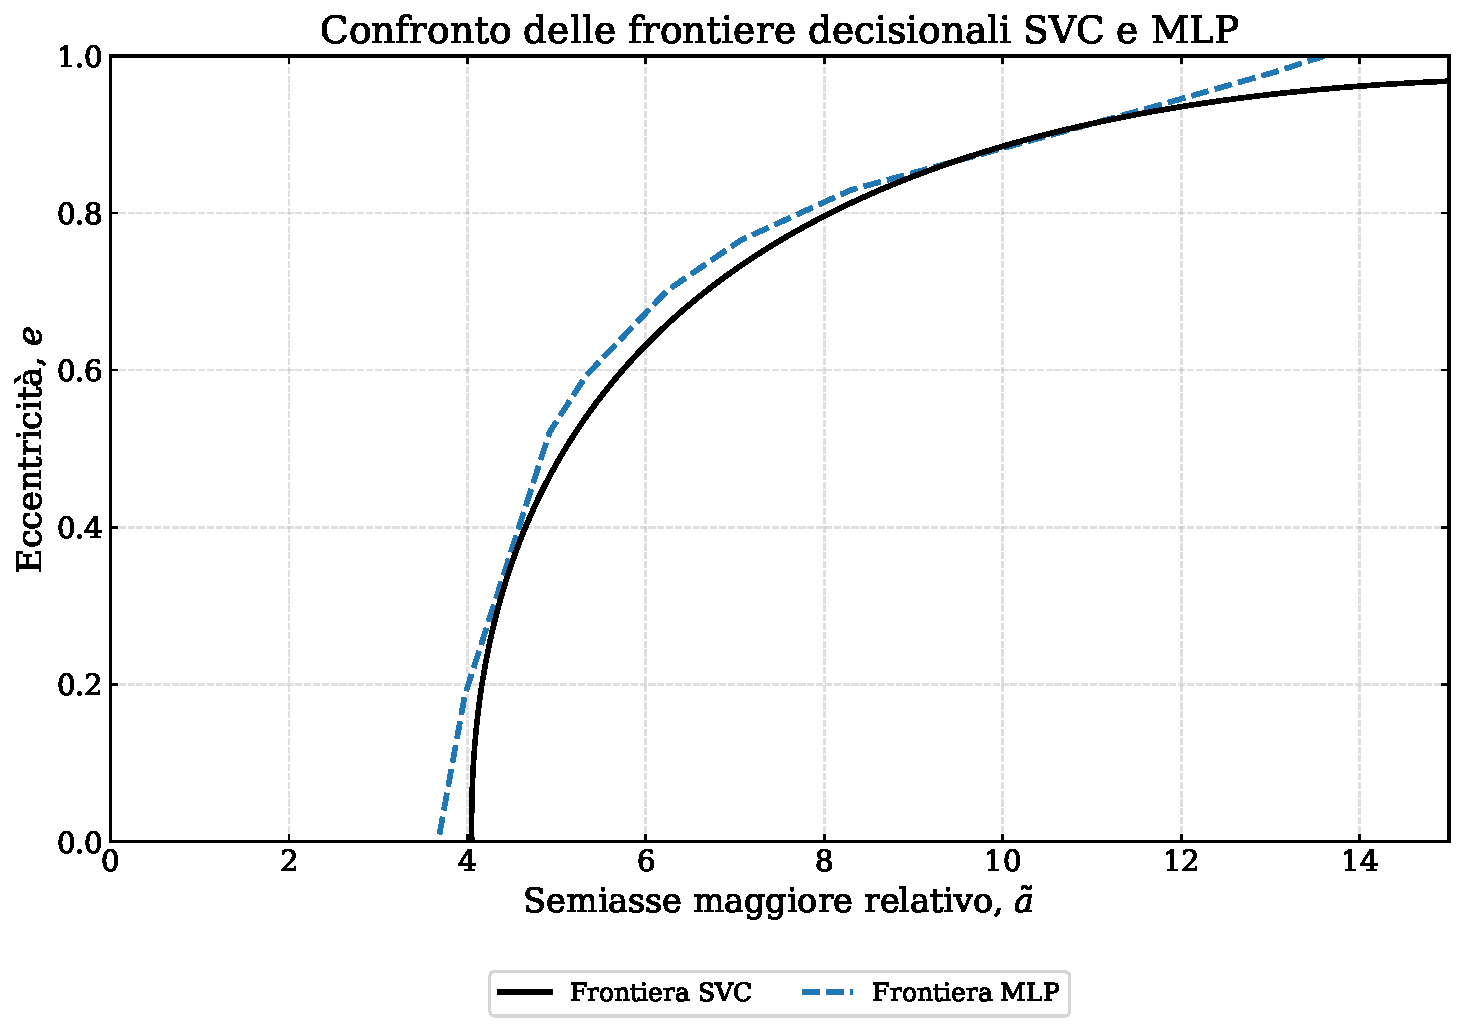
\includegraphics[width=0.7\textwidth]{./plots/svc_mlp_decision_boundaries.pdf}
	\caption{Comparison between the decision boundaries of the SVC (solid line) and MLP (dashed line) classifiers.}
	\label{fig:confronto-frontiere-svc-mlp}
\end{figure}%
